\section*{Part A}
\addcontentsline{toc}{section}{Part A}

\begin{tcolorbox}
  A.1) Provide the Matlab code required to synthesise the waveform in equation 12 and the resulting waveform.
\end{tcolorbox}

\lstinputlisting[
  caption = Requirement 1 MATLAB code,
  % captionpos = b,
  % firstline = 10,
  % lastline = 12,
  label = code:A_r,
]{matlab/A_r.m}

\begin{figure}[htbp]
  \centering
  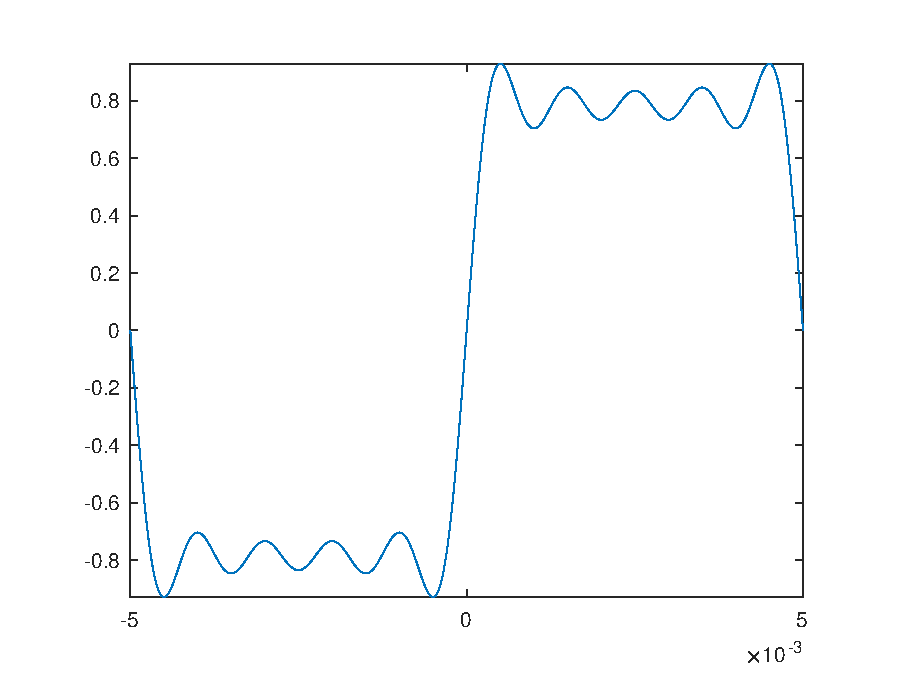
\includegraphics[width=0.8\textwidth]{matlab/fig/A_r.eps}
  \caption{waveform of $f(t) = V_o(\sin\omega t+\frac{1}{3}\sin3\omega t+\frac{1}{5}\sin5\omega t+\frac{1}{7}\sin7\omega t+\frac{1}{9}\sin9\omega t)$}    
  \label{fig:A_r}
\end{figure}

\begin{tcolorbox}
  A.2) Explain the features of the resulting waveform.
\end{tcolorbox}

The waveform is symmetric about the origin. Its peak-to-peak amplitude is $2V_{pp}$. It has ripples on the top and at the bottom. It is a periodic wave with a period of 0.01 seconds.

\pagebreak

\begin{tcolorbox}
  A.3) How do you think the waveform would look if an unlimited number of harmonics was available?
\end{tcolorbox}

\lstinputlisting[
  caption = Question 2 MATLAB code,
  label = code:A_q_2,
]{matlab/A_q_2.m}

\begin{figure}[hb]
  \centering
  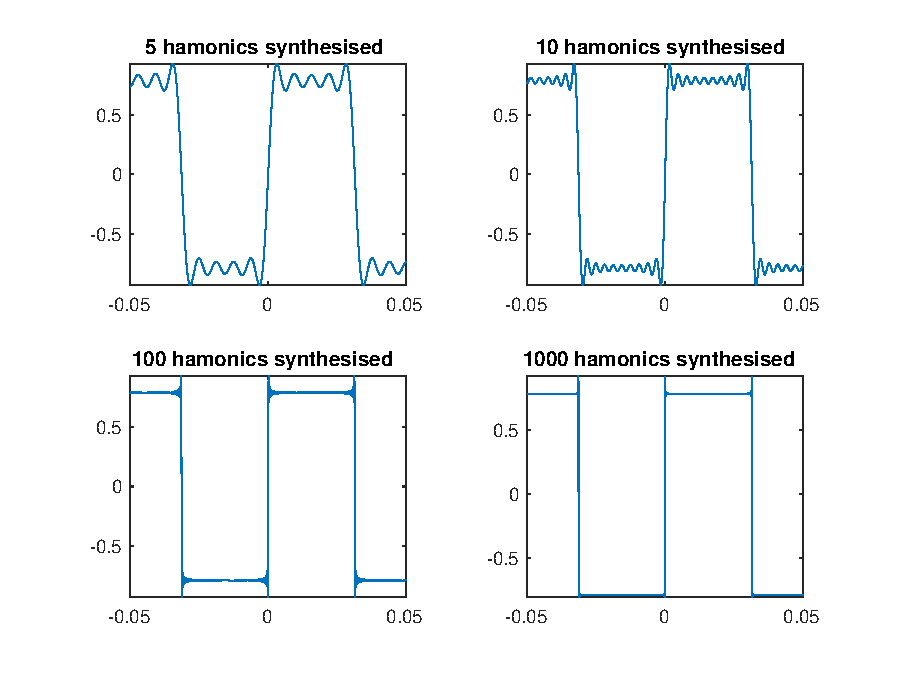
\includegraphics[width=0.79\textwidth]{matlab/fig/A_q_2.eps}
  \caption{As the number of harmonics increases, the resulting waveform gets closer to a square wave.}    
  \label{fig:A_q_2}
\end{figure}

If an unlimited number of harmonics was available, the wave form could be an ideal square wave.

\pagebreak

\begin{tcolorbox}
  A.4) Referring to Equation 3, what is the value of $a_o$?
\end{tcolorbox}

$a_o$ equals 0; because the wave is symmetric to the origin, so it does not have a value for dc term.

\begin{tcolorbox}
  A.5) Find an expression (in terms of n) for $a_n$ and $b_n$.
\end{tcolorbox}

The function is an odd function, so it does not have even components; hence $a_n$ equals 0.

After observation and induction, $b_n = \frac{1}{2n-1}$.

\begin{tcolorbox}
  A.6) Plot the spectrum (frequency domain view) of $f(t)$ using $c_n=\sqrt{a_n^2+b_n^2}$.
\end{tcolorbox}

\lstinputlisting[
  caption = Question 4 MATLAB code,
  label=code:A_q_4,
]{matlab/A_q_4.m}

\begin{figure}[htbp]
  \centering
  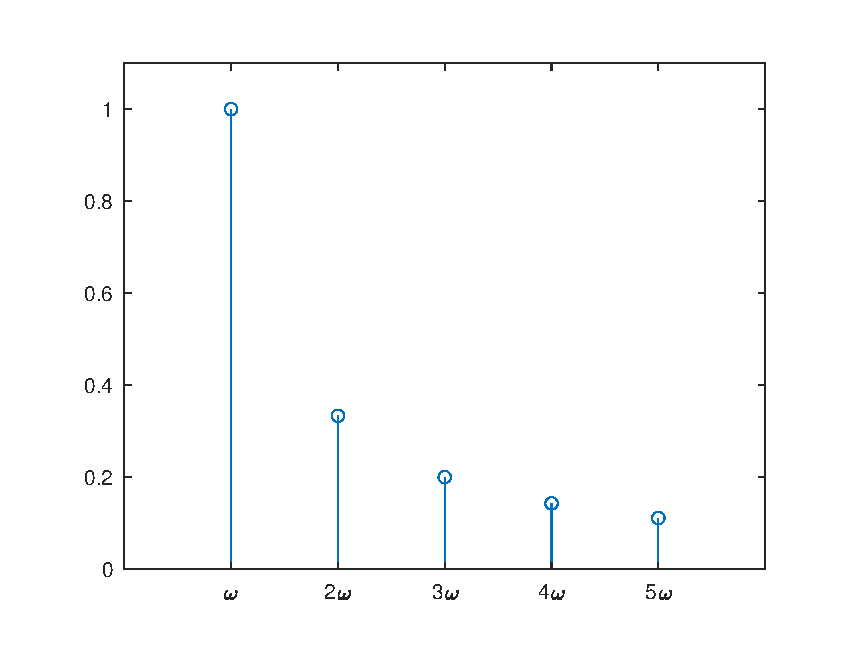
\includegraphics[width=0.8\textwidth]{matlab/fig/A_q_4.eps}
  \caption{the spectrum of $f(t)$ using $c_n=\sqrt{a_n^2+b_n^2}$}    
  \label{fig:A_q_4}
\end{figure}

\pagebreak